\documentclass[12pt]{article}
%\usepackage[utf8]{inputenc}
%\documentclass[UTF8]{ctexart}
%\usepackage[UTF8, heading = false, scheme = plain]{ctex}
\usepackage{geometry}
%geometry{a4paper,scale=0.9}
\geometry{a4paper,left=1cm,right=1cm,top=1cm,bottom=2cm}
\usepackage{amsfonts}
\usepackage{color}
\usepackage{url}
%\usepackage{biblatex}
\usepackage{amsmath}
\usepackage{amssymb}
\usepackage{latexsym}
\usepackage{cite}
%\addbibresource{ref.bib}
%\bibliography{ref.bib}
\usepackage{caption}
\usepackage{graphicx, subfig}
\usepackage{float}
%\usepackage[fontset=ubuntu]{ctex}
%\usepackage{fontspec}
\usepackage{xeCJK}
%\usepackage[colorlinks,
%anchorcolor=black,
%citecolor=black]{hyperref}
%\setmainfont{SimSun}
\usepackage[section]{placeins}
\usepackage{enumitem}
\usepackage{framed}
\usepackage[framemethod=TikZ]{mdframed}
\usepackage{indentfirst}
\usepackage{setspace}%使用间距宏包
\linespread{1.5}

\title{因果推断在阿里文娱用户增长中的应用\cite{Causal_Inference_In_Ali_User_Growth}}
\author{leolinuxer}
%\date{June 2020}

\begin{document}
%\setlength{\parindent}{0pt}
\maketitle
\tableofcontents

\section{导读}
如何实现产品的用户增长?显然,这是各家移动互联网应用的头等大事,也是悬在各家业务负责人头上的"天问"。在移动互联网进入下半场的大趋势下,过去粗放式的买量、厂商合作等模式越来越会受到掣肘,将更加依赖精细化的用户增长策略和产品用户体验的细致打磨;\textbf{经典的 AARRR 模式会逐步转向 RARRA 模式},提升产品留存、拉活、分享传播等方式是构建增长的主要战场。而在此之中,对于一个内容型产品,个性化算法对于用户留存、拉活将起到决定性的作用。

AARRR模型向RARRA模型的转换:
\begin{figure}[H]
    \centering
    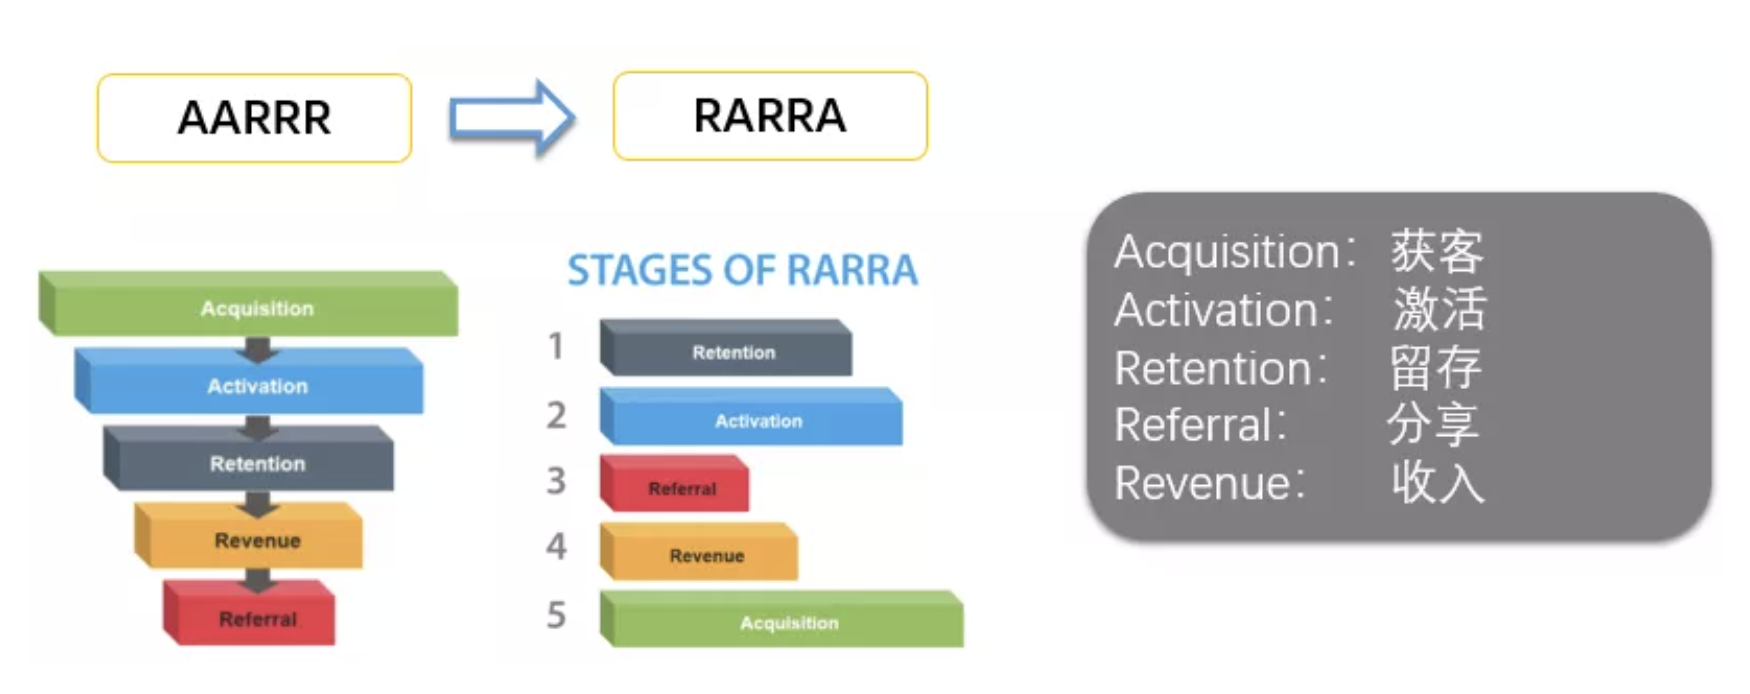
\includegraphics[width=1\textwidth]{fig/CasualInferenceInAli-User-Growth-Model.png}
    
\end{figure}
\begin{framed}
%\verb|\documentstyle[ifthen,12pt,titlepage]{article}|
也就是说,从“获客 -> 激活  -> 留存 -> 分享 -> 收入” 转为“留存 -> 激活 -> 分享 -> 收入 -> 获客”(参见扩展阅读)
\end{framed}

\section{相关背景}
考察与优酷类似的应用,在内容领域,增长的成功案例有:
\begin{itemize}
\setlength{\itemsep}{0pt}
\setlength{\parsep}{0pt}
\setlength{\parskip}{0pt}
    \item \textbf{“头条快手”模式}:内容分发类产品,代表是"今日头条"、"抖音"、"快手"等。\textbf{这类产品构建了完善的内容生产和消费生态,旨在通过推荐系统同时刺激生产和消费,实现两端的同时增长}。
    \item \textbf{“趣头条”模式}:该产品同属内容分发类产品,但较早地参考了网络游戏模式,\textbf{从各个环节设计用户里程碑和激励},不断引导新用户一步步完成点击、下刷、完整阅读、分享、关注等目标里程碑,并给予虚拟货币和真实货币的激励,在短时间内获取了大量下沉用户。
    \item \textbf{“爱奇艺”、“腾讯视频”模式}:这类产品利用大量资金和精准的内容采买眼光,\textbf{利用头部内容的流量聚集效应},在前几年迅速圈定大批用户,并形成长视频 app 特有用户心智。由于内容头部化,个性化算法在其中发挥的空间和作用较小,产品、模式趋于同质化,内容采买的巨大资金投入使得长视频网站的盈利遥遥无期。
\end{itemize}

会员增长是长视频产品体系下用户增长的特有子问题。优酷作为国内顶尖的视频内容提供商,上述三种增长模式都是需要进行借鉴的。\textbf{用户增长问题需要从内容供给、内容分发、权益设计、产品设计等多环节进行联合优化},从算法的角度,其目标可以拆解为两大部分:
\begin{itemize}
\setlength{\itemsep}{0pt}
\setlength{\parsep}{0pt}
\setlength{\parskip}{0pt}
    \item \textbf{用户状态建模}:深度建模用户状态和行为,从大数据集中找到使用户\textbf{从低阶状态到高阶状态转化的干预因子}。
    \item \textbf{个性化分发的升级}:将用户行为建模后,在多个场景\textbf{将这些干预动作落地为个性化推荐算法和营销算法},满足用户的视频内容消费需求。
\end{itemize}

阿里大文娱是阿里集团双 H 战略 ( Happiness \& Health ) 中最为重要的践行者,在不断为广大网民提供优质内容与良好体验的同时,我们也面临着用户规模化增长以及营收有计划提升的压力。我们已经逐步形成以\textbf{消息推送 ( push )、站外引导 ( dsp ) 以及新用户承接推荐等场景组成的用户增长业务体系},也已经逐步形成了\textbf{以权益发放 ( 营销 ) 以及商业化 ( 广告 ) 等抓手组成的收入增长业务体系}。基于因果推断的推荐算法、基于双 pid 的动态报价算法以及基于 uplift model 的营销增益模型正是应用在这两大业务体系中的,我们已经在多个业务场景中取得了较为显著的效果提升,我们相信其中的一些技术必将对整个互联网业内在增长算法体系带来一些崭新的视角、思考和实践经验。本文将主要为大家介绍基于因果推断的推荐算法。

\section{用户增长和智能营销算法的目标}
刚刚已经介绍了优酷用户增长的业务打法和构思,其中已经提到,个性化的分发算法是实现用户增长的主战场。其中有两大目标:
\begin{itemize}
\setlength{\itemsep}{0pt}
\setlength{\parsep}{0pt}
\setlength{\parskip}{0pt}
    \item \textbf{用户状态建模}:深度建模用户状态和行为,从大数据集中找到使用户\textbf{从低阶状态到高阶状态转化的干预因子}。
    \item \textbf{个性化分发的升级}:将用户行为建模后,在多个场景\textbf{将这些干预动作落地为个性化推荐算法和营销算法},满足用户的视频内容消费需求。
\end{itemize}

针对目标1,\textbf{传统数据分析主要是建模变量之间的相关性而非因果关系,不能从真正的因果关系来设计干预手段}。

针对目标2,\textbf{传统的推荐算法主要进行短期的点击、时长等多目标预估,未能从用户状态的跃迁去设计个性化的目标机制;其次目前大量应用的深度学习类算法同样属于统计学习派别的延展,其模型可解释性差},不能从中推断用户兴趣与内容的因果关系,而该类技术方向的演化会导致用户画像的算法较为单薄,不能满足优酷会员营销核心业务的需求。

基于因果推断的推荐算法我们已经成功应用在消息推送 ( push ) 以及 dsp 外投买量算法等业务中,而在营销场景中应用的 uplift 模型本质上也是因果推断思想的一个典型应用。因此,我们在整个用户增长以及智能营销的业务场景中逐步推广地应用了因果推断的思想,在某些实验中取得了非常好的业务结果,比如我们在 push 和 dsp 业务中的沉默用户召回这个场景下就取得了点击量和点击率的显著提升。

\subsection{用户状态表示}
\subsubsection{用户画像与状态表示法}
传统的用户画像表示技术要么服务于运营可解释性,要么服务于推荐或广告系统的模型预估,通常建模成向量 ( 离散高维或低维稠密 )。而我们在深入研究在线视频和付费会员业务后,发现\textbf{状态转移图}是更有力地建模该业务下用户画像的数据结构,原因如下:
\begin{itemize}
\setlength{\itemsep}{0pt}
\setlength{\parsep}{0pt}
\setlength{\parskip}{0pt}
    \item 用户从非会员到购买会员并逐步进入高阶会员的阶段,本质属于一种\textbf{强规则定义}的状态。
    \item 在线视频,尤其是长视频领域具备长时间、连续型消费 ( 追剧、追网红 ) 等特点,对比传统的图文推荐系统、电商推荐系统和广告系统,\textbf{用户的消费行为可以在连续的时间上进行切分,状态表示法是对向量表示法的有力补充}。
    \item 新用户的承接和推荐策略是用户增长中"促留存",建立心智的重要阶段。借鉴网络游戏和趣头条的思路,\textbf{将难度较大的"促留存"问题拆分为"目标达成"问题,产品通过策略不断使得用户完成高阶里程碑},是业内目前已证明成功的用户增长方法。
\end{itemize}

序中已经提到,\textbf{会员模式是长视频业务的核心付费模式},在用户的整个生命周期内,其大体的会员状态转移图如下:
\begin{figure}[H]
    \centering
    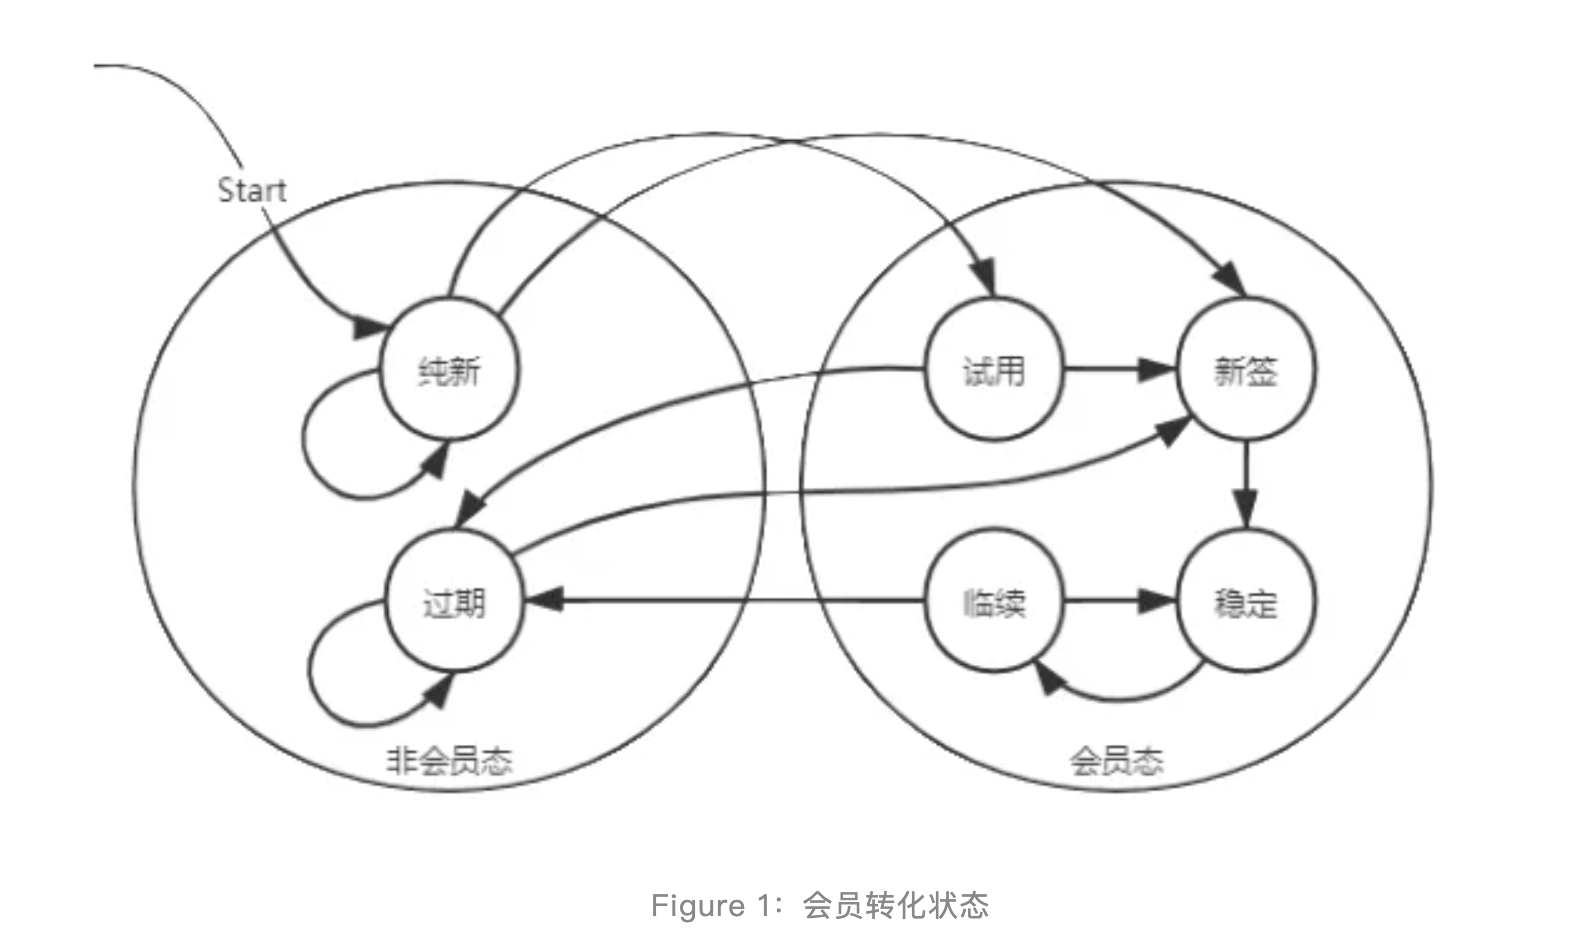
\includegraphics[width=1\textwidth]{fig/MemberStatusTransition.png}
\end{figure}

新用户阶段是产品对用户建立信任感的最重要时期,新用户在优酷 app 中的里程碑可以大致描述如下:
\begin{figure}[H]
    \centering
    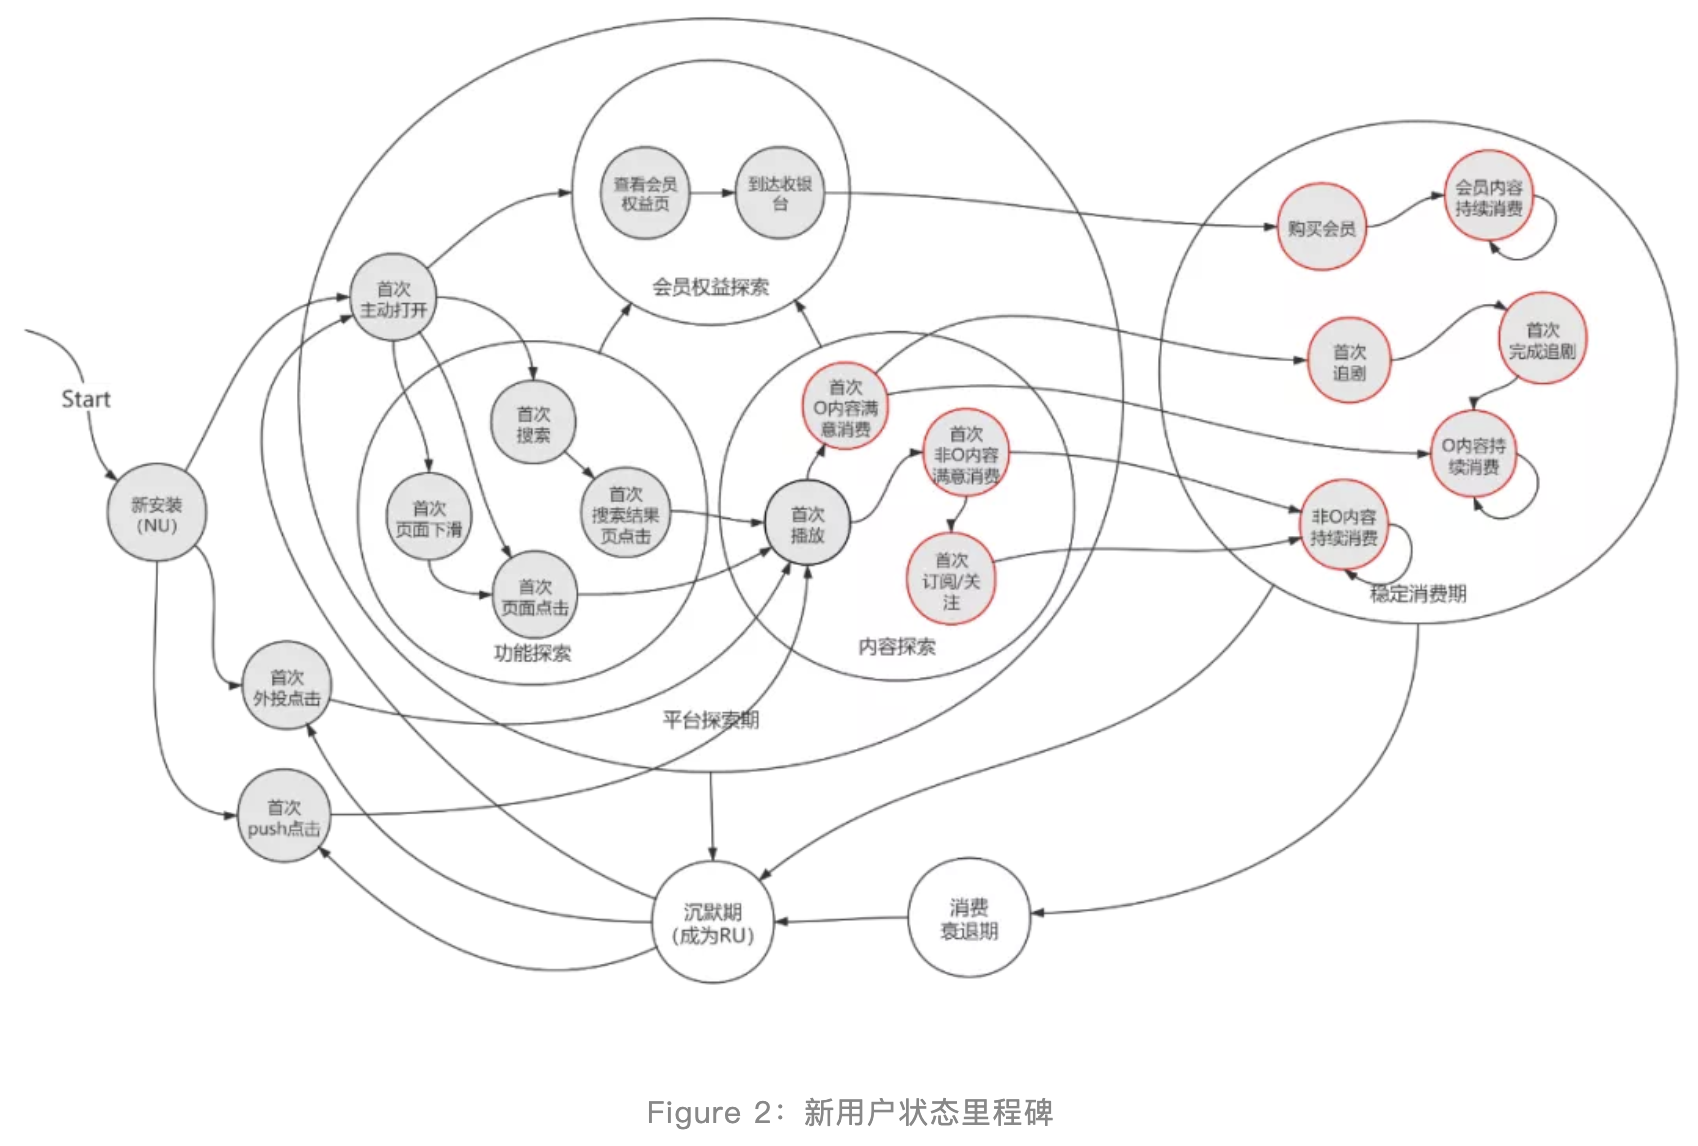
\includegraphics[width=1\textwidth]{fig/NewMemberStatusMilestones.png}
\end{figure}

可以看到,用户在不同的状态下,我们期望他们能完成\textbf{状态的"跃迁"},也就是从低阶状态不断往高阶状态:"持续消费","订阅/关注","追剧","会员稳定期"等转化。

可以预见的是,这种用户画像的表示方法,将会对业内长久以来已经趋于成熟的个性化推荐算法步向新的发展阶段:即为用户增长这个核心业务问题更好的服务。首先是多目标的排序机制,\textbf{对于在不同状态下的用户,个性化算法的机制目标会不同 ( 跃迁至目标态 )};其次启发我们从更前沿的算法高度来研究状态跃迁的干预手段问题,进而解决推荐系统中长期难解的"可解释性"、"幸存者偏差"、"兴趣探索"等问题。

针对干预手段的研究,在2019年用户增长 \& 智能营销团队组建之后,对因果推断 ( Causal Inference ) 算法率先进行了研究和落地,目前在个性化推送、外投 DSP 应用了基于 matching 的无偏 user-cf 算法,智能红包发放场景应用了 uplift model,取得了显著的核心业务指标提升,并得到了业务方和兄弟团队的一致认可。现将无偏 user-cf 算法介绍如下,uplift model 可参考文末推荐文章。

\section{基于因果推断的无偏 user-cf 设计}
\subsection{因果推断 ( Causal Inference ) 简介}
因果推断 ( Causal Inference ) 作为新兴的人工智能技术方向,旨在突破传统数据分析和机器学习方法的瓶颈,建模大规模数据集中的因果关系,为干预手段的设计提供指导,为构建下一代面向用户增长的全域分发系统提供理论基石。

因果推断的核心研究课题:
\begin{itemize}
\setlength{\itemsep}{0pt}
\setlength{\parsep}{0pt}
\setlength{\parskip}{0pt}
    \item 用户从非会员到购买会员并逐步进入高阶会员的阶段,本质属于一种\textbf{强规则定义}的状态。
    \item 从众多观测到/未观测到的变量中找出致因 ( causes )。
    \item 预估某个行为/因素的影响力/效益 ( causal effect )。
\end{itemize}

对于个体来说,核心是寻找反事实 ( counterfactual ) 镜像。在个性化推荐中,一个难题就是消除"幸存者"偏差(高活用户本身就容易受到推荐的影响),即如何将低活用户通过良好的路径推荐,逐步变成产品的高活用户。我们定义问题如下。

\subsection{建模过程}
\subsubsection{目标}
消去推荐系统的偏差。用户增长需要\textbf{消去高活用户带来的行为偏置,提升低活用户推荐效果}。

\subsubsection{假设}
用户变成低活、沉默的原因主要是因为对之前推荐不满意 ( 负例 )。

\subsubsection{方法}
 (1). 构建 Counterfactual 镜像人:利用无偏信息构造相似度量,构造低活 user 到高活 user 的 matching:
\begin{itemize}
\setlength{\itemsep}{0pt}
\setlength{\parsep}{0pt}
\setlength{\parskip}{0pt}
    \item 基础人口属性、安装的长尾 app 信息等
    \item 主动搜索行为 ( 非被动推荐 ),尤其是长尾 query
\end{itemize}

(2). 去除低活用户的 leave causes,推荐相似高活用户的 stay causes。对于推荐系统来说,这些 causes 包括:
\begin{itemize}
\setlength{\itemsep}{0pt}
\setlength{\parsep}{0pt}
\setlength{\parskip}{0pt}
    \item item 本身:但缺少泛化容易推出老内容
    \item item 的泛化特征:标签、时效性、质量
\end{itemize}

\begin{figure}[H]
    \centering
    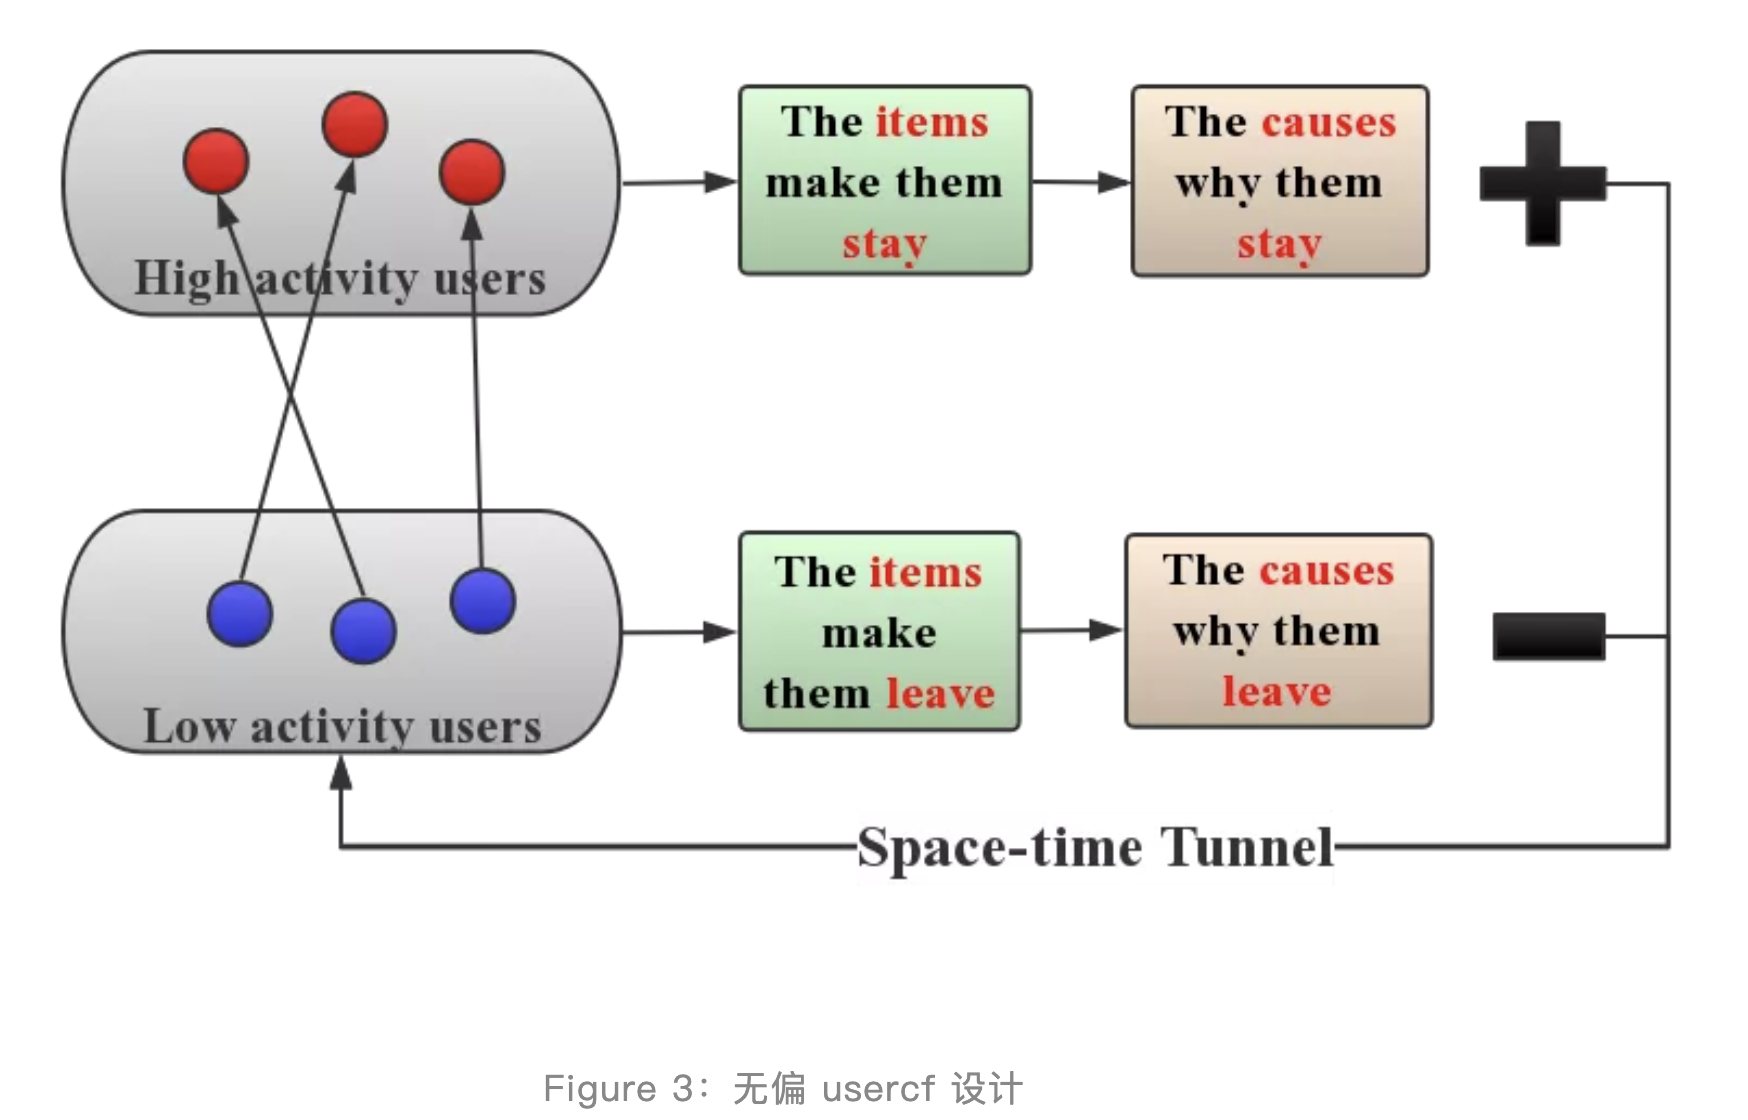
\includegraphics[width=1\textwidth]{fig/CasualInferenceInAli-User-CF.png}
\end{figure}

注意,由于使用了 matching 方法,这里的算法非常类似传统的 user-cf 类算法,但是和传统 user-cf 核心的区别在于:
\begin{itemize}
\setlength{\itemsep}{0pt}
\setlength{\parsep}{0pt}
\setlength{\parskip}{0pt}
    \item matching 不使用被动推荐数据,个性化推送、站内推荐、运营推荐的内容都不使用。
    \item 只匹配低活到高活,活跃度相同的用户之间不进行匹配。
\end{itemize}

\begin{framed}
几个要点的理解:

(1)用户集的一类重要的特征:低活和高活;

(2) 研究目标:研究什么样的推荐能够更好地将\textbf{低活}用户向\textbf{高价值}会员转化;

(3) 其中碰到的问题是:用户天然可分为低活和高活两类;如果直接对所有用户做 AB 实验,则实验组中的高活用户会影响实验结论(拉升推荐效果),导致我们无法针对性分析具体什么样的推荐内容,真正对低活用户是有效果的。

(4) 解决上述问题的方法是:将用户分为低活和高活两类;利用无偏信息构造相似度量,构造低活 user 到高活 user 的 matching:从而消去推荐系统的偏差。用户增长需要消去高活用户带来的行为偏置,提升低活用户推荐效果。

(5)参照上图,对比低活用户和高活用户收到了哪些因素的影响,导致了它们的后续行为出现了区别;
\end{framed}

\subsubsection{业务收益}
该算法落地后,在两个 baseline 相对较高的算法场景中取得了较大的收益:其中个性化推送 ( push ),在沉默用户中获得了 50%+ ctr 和 50%+ click 的双增长,在外投 dsp 业务中,拉活量对比峰值接近翻倍。

\section{总结与展望}
目前算法的应用,只是对应了两个用户状态 ( 低活->高活 ) 之间的推断,如 Figure 1 和 Figure 2 所描述的,用户增长的目标是将细分的低阶状态往高阶目标态上进行跃迁,那么该类算法很显然将会在数据分析、产品设计、分发优化等各个环节发挥巨大作用。整个2019年团队的实践虽然取得了很大的业务效果,但只是对该算法方向相对较浅显的应用,且对于优酷整体的增长问题来说,应用的场景还不够多,未来期望在其基础理论和实践都投入更多的资源。

可以预见的是:对于整个业内用户增长的方法论,该方法在未来必将成为核心的理论基石。对于个性化推荐这一经典领域,该方法为解决经典难题"幸存者偏差","可解释性","用户表示","兴趣探索"等提供了漂亮的解法。

\section{扩展知识}
\subsection{AARRR模型}
\begin{itemize}
\setlength{\itemsep}{0pt}
\setlength{\parsep}{0pt}
\setlength{\parskip}{0pt}
    \item Acquisition:  获客
    \item Activation: 激活
    \item Retention: 留存
    \item Referral: 分享
    \item Revenue: 收入
\end{itemize}

\subsection{幸存者偏差(Survivorship Bias)}
幸存者偏差(Survivorship bias)是一种常见的逻辑谬误,意思是没有考虑到筛选的过程,忽略了被筛选掉的关键信息,只看到经过筛选后而产生的结果。

一个例子是在做统计分析时,我们只专注于那些成功的例子,从而得出以偏概全的错误结论。大致来讲,成功的例子往往只属于少数。如果我们只看成功的幸存者,而忽略那些大部分的“倒霉蛋”,那么就会得出很多不符合常理的荒唐结论。

思考:在弹孔最密集的部分加上装甲,能提高飞机的防御能力吗?答案是不能,因为这些百孔千疮的轰炸机是从战场上成功飞回来的“幸存者”,因此它们机身上的弹孔对于飞机来说算不上致命。要想救那些轰炸机飞行员的性命,更正确的方法应该是去研究那些被打中并坠毁的轰炸机。

\textbf{幸存者偏差直接影响的就是新产品的功能迭代}。功能迭代一般都从最容易收集到反馈的用户那里获得。通过询问 the current top users 最希望在产品中看到哪些改进,从而构建新功能。但是,这可能完全忽略了目标市场中那部分没有给你任何数据的人对你的产品不感兴趣的原因。就像被击落的飞机无法告诉你它是怎么死的。

\textbf{如何应对?}——让每一架飞机都尽可能飞回来。
\begin{itemize}
\setlength{\itemsep}{0pt}
\setlength{\parsep}{0pt}
\setlength{\parskip}{0pt}
    \item 计算出目标市场中哪些部分没有反馈。比如说通过查看当前用户在目标市场所处的位置,以及我们如何获得这部分用户来反向推导

    \item 想办法收集并联系我们曾经触及过但并未成功转换的用户(比如说访问过网站但并没有试用产品的人群)

    \item 针对上图中的每个步骤制定相应措施,根据这些对产品不感兴趣的人群重新制定营销策略或者产品改进
\end{itemize}




\section{扩展阅读}
RARRA 模型(\url{https://36kr.com/p/1722896957441})

\url{http://www.woshipm.com/operate/1518912.html}

\url{http://www.woshipm.com/operate/3037467.html}

因果推断

\url{https://mp.weixin.qq.com/s/rSnS0r_6YWCT2o6fD15uEw}

"可解释性"、"兴趣探索"

基于双 pid 的动态报价算法(\url{https://mp.weixin.qq.com/s?__biz=MzU1NTMyOTI4Mw==&mid=2247498041&idx=1&sn=5c8b880a2be4075ee48388b27ce1a6e0&chksm=fbd74b55cca0c24382f3f10e6f2a8423e228c390339dc086d5f1fec034350e0574302587834a&scene=21#wechat_redirect})

%\printbibliography
\bibliography{../ref}
\bibliographystyle{IEEEtran}
\end{document}